\documentclass[aspectratio=169]{../latex_main/tntbeamer}  % you can pass all options of the beamer class, e.g., 'handout' or 'aspectratio=43'
\usepackage{dsfont}
\usepackage{bm}
\usepackage[english]{babel}
\usepackage[T1]{fontenc}
%\usepackage[utf8]{inputenc}
\usepackage{graphicx}
\graphicspath{ {./figures/} }
\usepackage{algorithm}
\usepackage[ruled,vlined,algo2e,linesnumbered]{algorithm2e}
\usepackage{hyperref}
\usepackage{booktabs}
\usepackage{mathtools}

\usepackage{amsmath,amssymb}

\DeclareMathOperator*{\argmax}{arg\,max}
\DeclareMathOperator*{\argmin}{arg\,min}

\usepackage{amsbsy}
\newcommand{\vect}[1]{\bm{#1}}
%\newcommand{\vect}[1]{\boldsymbol{#1}}

\usepackage{pgfplots}
\pgfplotsset{compat=1.16}
\usepackage{tikz}
\usetikzlibrary{trees} 
\usetikzlibrary{shapes.geometric}
\usetikzlibrary{positioning,shapes,shadows,arrows,calc,mindmap}
\usetikzlibrary{positioning,fadings,through}
\usetikzlibrary{decorations.pathreplacing}
\usetikzlibrary{intersections}
\pgfdeclarelayer{background}
\pgfdeclarelayer{foreground}
\pgfsetlayers{background,main,foreground}
\tikzstyle{activity}=[rectangle, draw=black, rounded corners, text centered, text width=8em]
\tikzstyle{data}=[rectangle, draw=black, text centered, text width=8em]
\tikzstyle{myarrow}=[->, thick, draw=black]

% Define the layers to draw the diagram
\pgfdeclarelayer{background}
\pgfdeclarelayer{foreground}
\pgfsetlayers{background,main,foreground}

% Requires XeLaTeX or LuaLaTeX
%\usepackage{unicode-math}

\usepackage{fontspec}
%\setsansfont{Arial}
\setsansfont{RotisSansSerifStd}[ 
Path=../latex_main/fonts/,
Extension = .otf,
UprightFont = *-Regular,  % or *-Light
BoldFont = *-ExtraBold,  % or *-Bold
ItalicFont = *-Italic
]
\setmonofont{Cascadia Mono}[
Scale=0.8
]

% scale factor adapted; mathrm font added (Benjamin Spitschan @TNT, 2021-06-01)
%\setmathfont[Scale=1.05]{Libertinus Math}
%\setmathrm[Scale=1.05]{Libertinus Math}

% other available math fonts are (not exhaustive)
% Latin Modern Math
% XITS Math
% Libertinus Math
% Asana Math
% Fira Math
% TeX Gyre Pagella Math
% TeX Gyre Bonum Math
% TeX Gyre Schola Math
% TeX Gyre Termes Math

% Literature References
\newcommand{\lit}[2]{\href{#2}{\footnotesize\color{black!60}[#1]}}

%%% Beamer Customization
%----------------------------------------------------------------------
% (Don't) Show sections in frame header. Options: 'sections', 'sections light', empty
\setbeamertemplate{headline}{empty}

% Add header logo for normal frames
\setheaderimage{
	% 
\includegraphics[height=\logoheight]{figures/TNT_darkv4.pdf}
	
\includegraphics[height=\logoheight]{../latex_main/figures/luh_logo_rgb_0_80_155.pdf}
	% 
\includegraphics[height=\logoheight]{figures/logo_tntluh.pdf}
}

% Header logo for title page
\settitleheaderimage{
	% 
\includegraphics[height=\logoheight]{figures/TNT_darkv4.pdf}
	
\includegraphics[height=\logoheight]{../latex_main/figures/luh_logo_rgb_0_80_155.pdf}
	% 
\includegraphics[height=\logoheight]{figures/logo_tntluh.pdf}
}

% Title page: tntdefault 
\setbeamertemplate{title page}[tntdefault]  % or luhstyle
% Add optional title image here
%\addtitlepageimagedefault{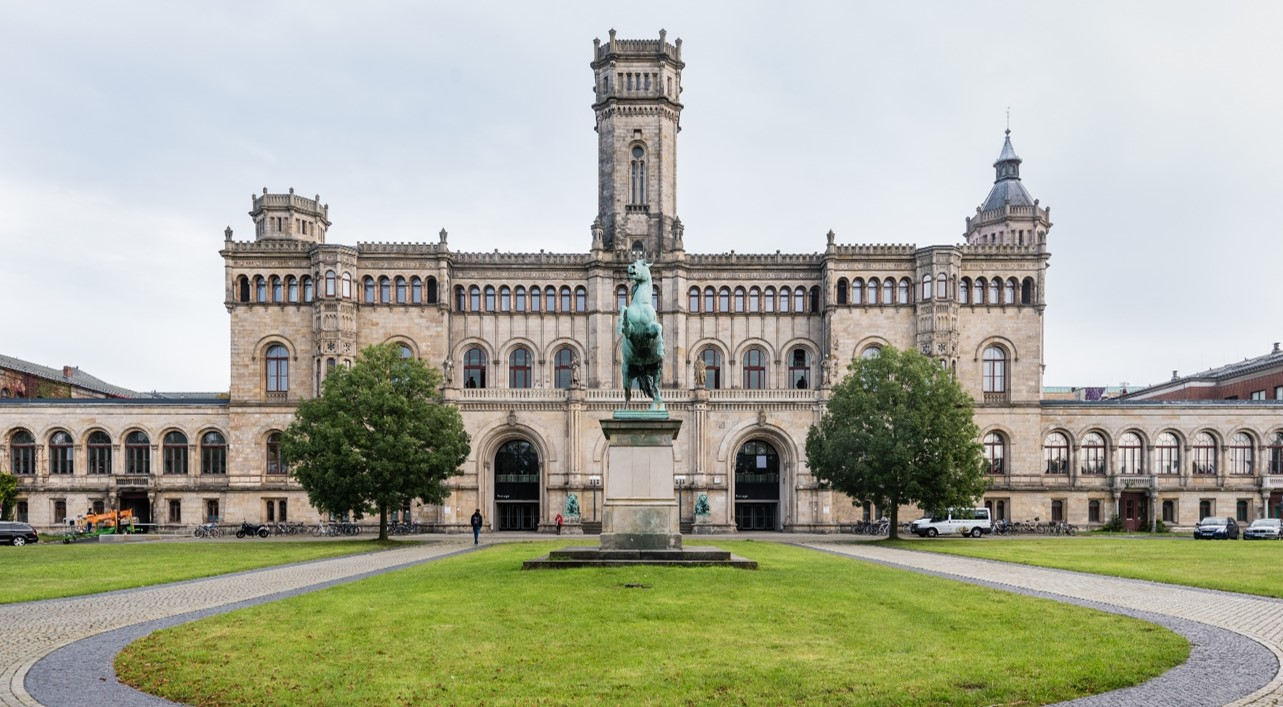
\includegraphics[width=0.65\textwidth]{figures/luh_default_presentation_title_image.jpg}}

% Title page: luhstyle
% \setbeamertemplate{title page}[luhstyle]
% % Add optional title image here
% \addtitlepageimage{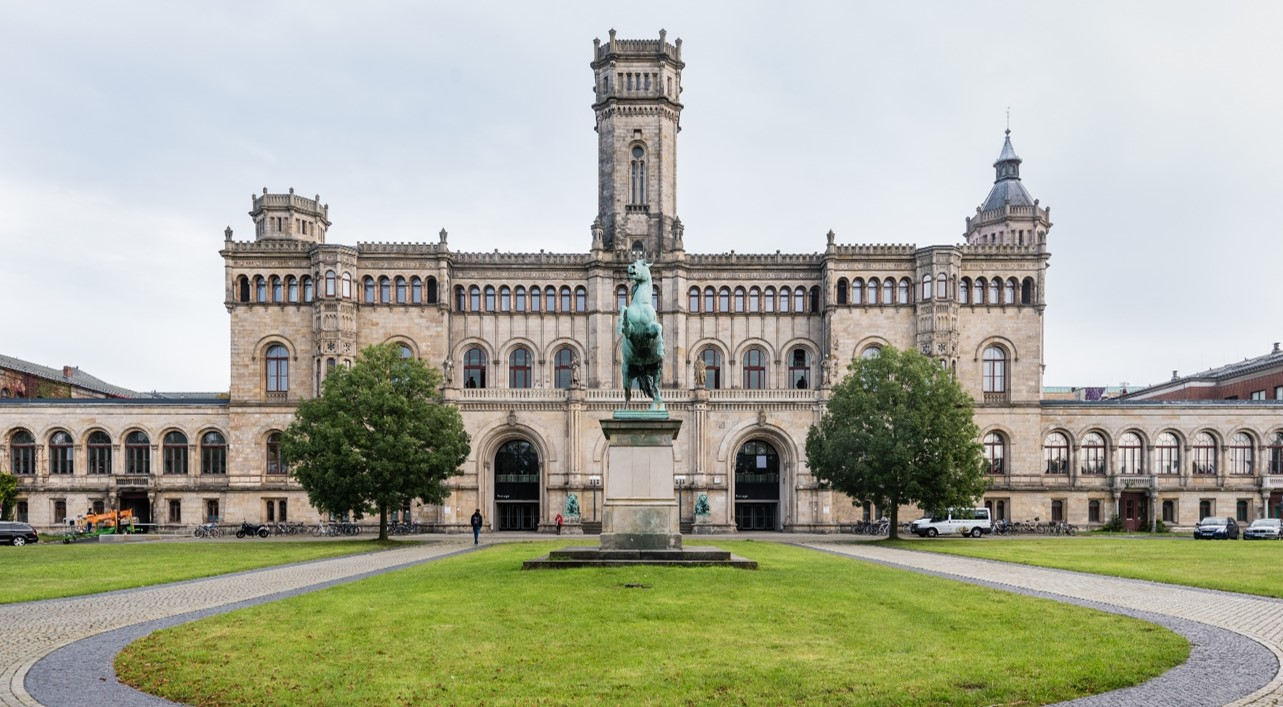
\includegraphics[width=0.75\textwidth]{figures/luh_default_presentation_title_image.jpg}}

\author[Abedjan \& Lindauer]{Ziawasch Abedjan \& Marius Lindauer\\[1em]
	
\includegraphics[height=\logoheight]{../latex_main/figures/luh_logo_rgb_0_80_155.pdf}\qquad
	
\includegraphics[height=\logoheight]{../latex_main/figures/DBIS_Kurzlogo.png}\qquad

\includegraphics[height=\logoheight]{../latex_main/figures/TNT_darkv4}\qquad

\includegraphics[height=\logoheight]{../latex_main/figures/L3S.jpg}	}
\date{Summer Term 2022; \hspace{0.5em} {
\includegraphics[height=1.5em]{../latex_main/figures/Cc-by-nc-sa_icon.svg.png}}; based on \href{https://ds100.org/fa21/}{[DS100]}
}


%%% Custom Packages
%----------------------------------------------------------------------
% Create dummy content
\usepackage{blindtext}

% Adds a frame with the current page layout. Just call \layout inside of a frame.
\usepackage{layout}


%%% Macros
%\renewcommand{\vec}[1]{\mathbf{#1}}
% \usepackage{bm}
%\let\vecb\bm

\title[Introduction]{DS: Introduction}
\subtitle{What is data science?}

\graphicspath{ {./figure/} }
%\institute{}


\begin{document}
	
	\maketitle

    \begin{frame}{Data is changing the world}
        \begin{figure}
            \centering
            \includegraphics[scale= .65]{bild1}
        \end{figure}
    \end{frame}

    % \begin{frame}{Data science is a fundamentally interdisciplinary field}
    %     \begin{figure}
    %         \centering
    %         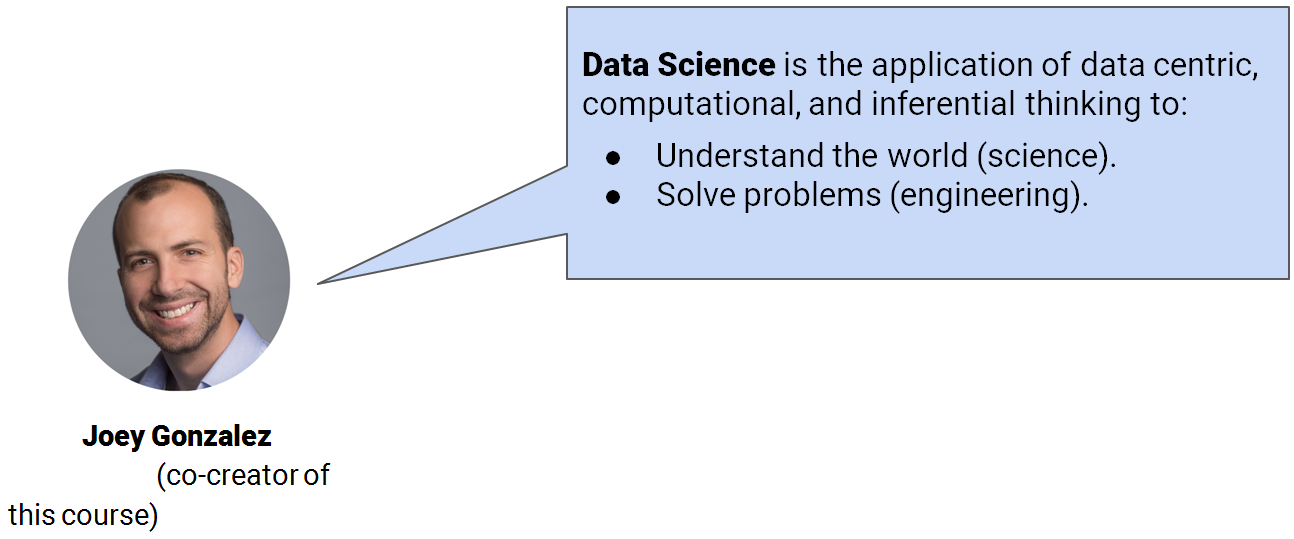
\includegraphics[scale=.43]{bild2}
    %     \end{figure}
    % \end{frame}

    \begin{frame}{Data Science Venn Diagram}
        \begin{figure}
            \centering
            \includegraphics[scale=.4]{bild3}
        \end{figure}
    \end{frame}

    \begin{frame}{Data Science in Industry}
        \begin{figure}
            \centering
            \vspace{-2em}
            \includegraphics[scale= .65]{bild5}
        \end{figure}
        %The tasks that data scientists say they work on regularly.\\
        Self-reported. Based on the results of Kaggle’s 2019 Machine Learning \& Data Science Survey.
    \end{frame}
    
    \begin{frame}[c]{Insight}
        \begin{columns}
        \begin{column}{.5\textwidth}
        
        Good data analysis is not:
        \begin{itemize}
            \item Simple application of a statistics recipe.
            \item Simple application of statistical software.
        \end{itemize}
        There are many tools out there for data science, but they are merely tools.
        \begin{itemize}
            \item They don’t do any of the important thinking!
        \end{itemize}
        \end{column}
        \begin{column}{.4\textwidth}
        
            \begin{figure}
                \centering
                \includegraphics[width=1.0\textwidth]{bild4}
            \end{figure}
            
        \end{column}
        
        
        \end{columns}
        \bigskip
        “The purpose of computing is insight, not numbers.” - R. Hamming. Numerical Methods for Scientists and Engineers (1962).

    \end{frame}
    
    
    \begin{frame}[c]{Example questions in data science}
        Some (broad) questions we might try to answer with data science:
        \begin{itemize}
            \item Is the world getting better or worse?
            \item Is the use of the COMPAS algorithm for prison sentencing fair?
            \item Where should we put docking ports for our bikes?
            \item What should we eat to avoid dying early of heart disease?
            \item Do immigrants from poor countries have a positive or negative impact on the economy?
            \item Are people vaccinated against COVID-19 also protected from new variants
            \item Who will win the next soccer tournament?
        \end{itemize}
    \end{frame}
    
    
    \begin{frame}{Data science drives policy and public understanding}
        There are real-world implications of the work we do as data scientists.
        \begin{columns}
            \begin{column}{.6\textwidth}
                    \begin{figure}
                        \centering
                        \includegraphics[scale=.5]{bild6}
                    \end{figure}
                    The problem is that this weekly cycle is fake. It's an artifact of how the data is collected and reported.
            \end{column}
            
            \begin{column}{.4\textwidth}
                    \begin{figure}
                        \centering
                        \includegraphics[scale=.5]{bild7}
                    \end{figure}
            \end{column}
        \end{columns}
    \end{frame}
    
    \begin{frame}{Data science drives policy and public understanding}
        There are real-world implications of the work we do as data scientists.
        \begin{columns}
            \begin{column}{.3\textwidth}
                    \begin{figure}
                        \centering
                        \includegraphics[scale=.6]{bild8}
                    \end{figure}
            \end{column}
            \begin{column}{.3\textwidth}
                    \begin{figure}
                        \centering
                        \includegraphics[scale=.4]{bild9}
                    \end{figure}
            \end{column}
            
            \begin{column}{.3\textwidth}
                    \begin{figure}
                        \centering
                        \includegraphics[scale=.5]{bild10}
                    \end{figure}
            \end{column}
        \end{columns}
    \end{frame}


    \begin{frame}{Unconscious bias is real – be mindful of it}
    \begin{columns}
        \begin{column}{.4\textwidth}
            A “depixelizer” (link in description) was built that takes pixelated images and generates images that are perceptually realistic and downscale correctly.
            \begin{figure}
                \centering
                \includegraphics[scale=.5]{bild11}
            \end{figure}
        \end{column}
        \begin{column}{.4\textwidth}
            \begin{figure}
                \centering
                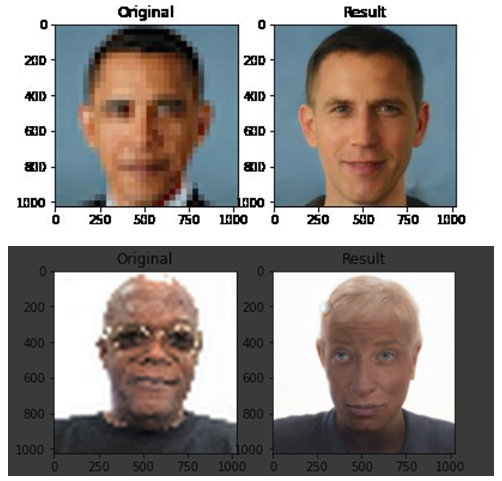
\includegraphics[scale=.37]{bild12}
            \end{figure}
            What do you notice? Why might this be happening?
        \end{column}
    \end{columns}
    
    \end{frame}
    
    \begin{frame}{Question what you see}
        \begin{columns}
            \begin{column}{.4\textwidth}
                    \begin{figure}
                        \centering
                        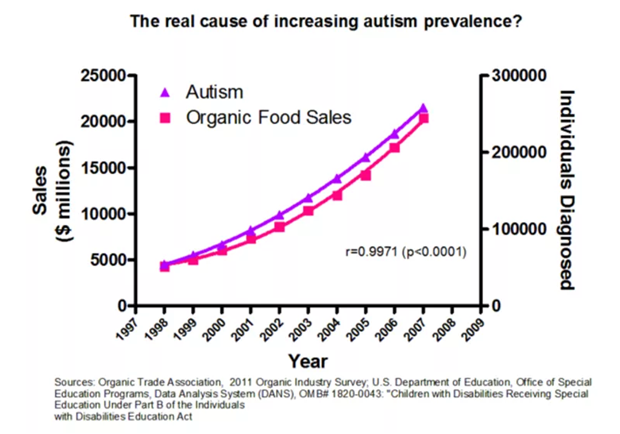
\includegraphics[scale=.5]{Bild13}
                    \end{figure}
                    Are autism rates and organic food sales inherently related? Seems unlikely.
            \end{column}
            
             \begin{column}{.4\textwidth}
                \begin{figure}
                    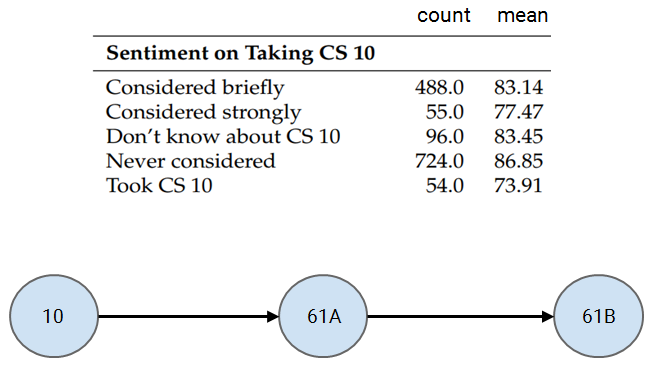
\includegraphics[scale=.35]{bild14}
                \end{figure}
                  Can taking a CS class make you worse at CS? Seems unlikely.
             \end{column}
           
        \end{columns}
    \end{frame}
    
    
\end{document}